\documentclass[11pt]{article} % use larger type; default would be 10pt

\usepackage{tikz}
\usetikzlibrary{calc}
\usetikzlibrary{arrows.meta}

        \newcommand\degree[0]{^{\circ}}

\title{Play with TikZ}
\author{Just Us}
%\date{} % Activate to display a given date or no date (if empty),
         % otherwise the current date is printed 

\begin{document}
\maketitle


\section{Chapter 2 review problems}


hp2-sum-7ans
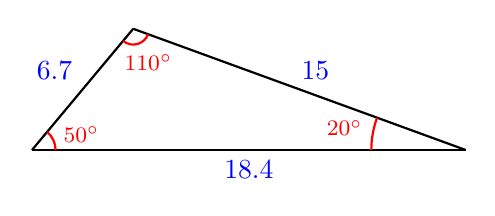
\begin{tikzpicture} 

\coordinate (A) at (0,0);
\coordinate (B) at (1.286,1.54);
\coordinate (C) at (5.51,0);

\draw[black,thick] (A)--(B) node[above left, midway] {\color{blue}$6.7$};
\draw[black,thick] (A)--(C) node[below, midway] {\color{blue}$18.4$};
\draw[black,thick] (C)--(B) node[above right, midway, xshift=-3] {\color{blue}$15$};

\draw[red,thick] (A)++(0.3,0) arc(0:50: 0.3) node[right, midway, yshift=2] {\footnotesize$50\degree$};
\draw[red,thick] (C)++(-1.2,0) arc(180:160: 1.2) node[left, midway, yshift=2] {\footnotesize$20\degree$};
\draw[red,thick] (B)++(-.1286,-.154) arc(-130:-20: 0.2) node[below, midway, xshift=4] {\footnotesize$110\degree$};

\end{tikzpicture}
\newline


revchap2.9
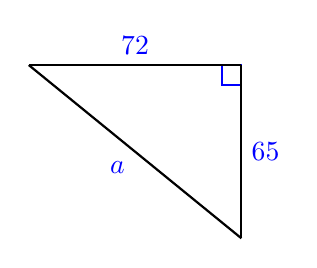
\begin{tikzpicture}

\coordinate (C) at (0,0 );
\coordinate (A) at (-2.7,0);
\coordinate (B) at (0,-2.2);

\draw[blue,thick] (C) rectangle +(-0.25,-0.25);

\draw[black,thick](C)--(A) node[above,midway] {\color{blue}$72$};
\draw[black,thick](C)--(B) node[right,midway] {\color{blue}$65$};
\draw[black,thick](A)--(B) node[below left,midway] {\color{blue}$a$};

\end{tikzpicture}
\newline

revchap2.10
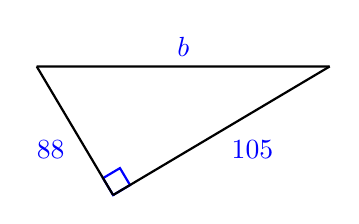
\begin{tikzpicture} [rotate=30.7]

\coordinate (C) at (0,0 );
\coordinate (A) at (3.2,0);
\coordinate (B) at (0,1.9);

\draw[blue,thick] (C) rectangle +(0.25,0.25);

\draw[black,thick](C)--(A) node[below right,midway] {\color{blue}$105$};
\draw[black,thick](C)--(B) node[below left,midway] {\color{blue}$88$};
\draw[black,thick](A)--(B) node[above,midway] {\color{blue}$b$};

\end{tikzpicture}
\newline

revchap2.11
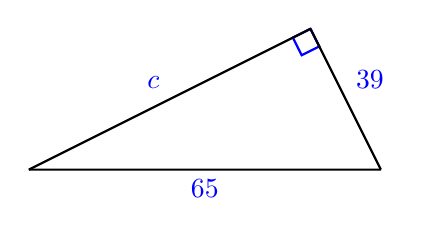
\begin{tikzpicture} [rotate=206.565]

\coordinate (C) at (0,0 );
\coordinate (A) at (4,0);
\coordinate (B) at (0,2);

\draw[blue,thick] (C) rectangle +(0.25,0.25);

\draw[black,thick](C)--(A) node[above left,midway] {\color{blue}$c$};
\draw[black,thick](C)--(B) node[above right,midway] {\color{blue}$39$};
\draw[black,thick](A)--(B) node[below,midway] {\color{blue}$65$};

\end{tikzpicture}
\newline

revchap2.12
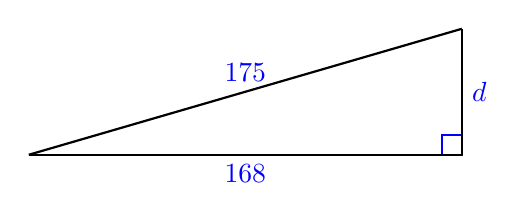
\begin{tikzpicture} 

\coordinate (C) at (0,0 );
\coordinate (A) at (-5.5,0);
\coordinate (B) at (0,1.6);

\draw[blue,thick] (C) rectangle +(-0.25,0.25);

\draw[black,thick](C)--(A) node[below,midway] {\color{blue}$168$};
\draw[black,thick](C)--(B) node[right,midway] {\color{blue}$d$};
\draw[black,thick](A)--(B) node[above ,midway] {\color{blue}$175$};


\end{tikzpicture}
\newline

revchap2.15
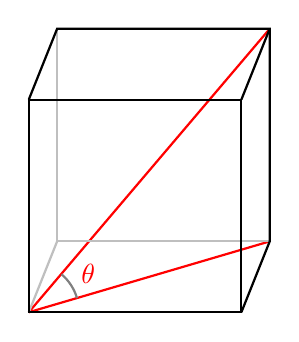
\begin{tikzpicture}  [scale=0.9]

\coordinate (O) at (0,0 );
\coordinate (A) at (3,0);
\coordinate (B) at (3,3);
\coordinate (C) at (0,3);

\coordinate (D) at (0.4,1);
\coordinate (E) at (3.4,1);
\coordinate (F) at (3.4,4);
\coordinate (G) at (0.4,4);

\draw[red,thick](O)--(E);
\draw[red,thick](O)--(F);
\draw[gray!50!white,thick](O)--(D);
\draw[gray!50!white,thick](G)--(D)--(E);
\draw[black,thick](A)--(E)--(F)--(G)--(C);
\draw[black,thick](B)--(F);
\draw[black,thick](A)--(B)--(C)--(O)--cycle;

\draw[gray,thick] (.68,.2) arc({atan(1/3.4)}:{atan(4/3.4)}:.7) node[above right,midway, yshift=-3]{\color{red}$\theta$};

\end{tikzpicture}
\newline

revchap2.16
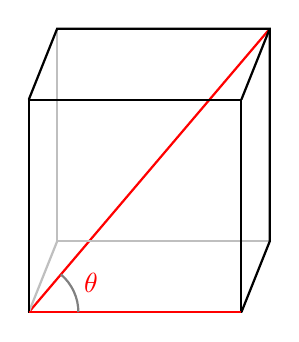
\begin{tikzpicture} [scale=0.9]

\coordinate (O) at (0,0 );
\coordinate (A) at (3,0);
\coordinate (B) at (3,3);
\coordinate (C) at (0,3);

\coordinate (D) at (0.4,1);
\coordinate (E) at (3.4,1);
\coordinate (F) at (3.4,4);
\coordinate (G) at (0.4,4);

\draw[red,thick](O)--(F);
\draw[gray!50!white,thick](O)--(D);
\draw[gray!50!white,thick](G)--(D)--(E);
\draw[black,thick](A)--(E)--(F)--(G)--(C);
\draw[black,thick](B)--(F);
\draw[black,thick](A)--(B)--(C)--(O)--cycle;

\draw[red,thick](O)--(A);
\draw[gray,thick] (.7,0) arc(0:{atan(4/3.4)}:.7) node[above right,midway, yshift=-4]{\color{red}$\theta$};

\end{tikzpicture}
\newline

revchap2.17
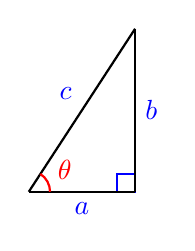
\begin{tikzpicture} [scale=0.9]

\coordinate (O) at (0,0 );
\coordinate (A) at (-1.5,0);
\coordinate (B) at (0,2.3);

\draw[blue,thick] (O) rectangle +(-0.25,0.25);
\draw[black,thick](B)--(O) node[right,midway] {\color{blue}$b$};
\draw[black,thick](A)--(B) node[above left,midway] {\color{blue}$c$};
\draw[black,thick](A)--(O) node[below,midway] {\color{blue}$a$};

\draw[red,thick] (A)++(.3,0) arc(0:{atan(2.3/1.5)}:.3) node[above right,midway, yshift=-3]{\color{red}$\theta$};

\end{tikzpicture}
\newline

revchap2.19
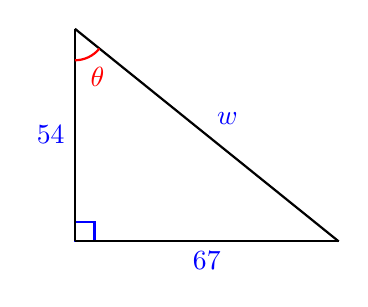
\begin{tikzpicture}

\coordinate (O) at (0,0 );
\coordinate (A) at (3.35,0);
\coordinate (B) at (0,2.7);

\draw[blue,thick] (O) rectangle +(0.25,0.25);
\draw[black,thick](B)--(O) node[left,midway] {\color{blue}$54$};
\draw[black,thick](A)--(B) node[above right,midway] {\color{blue}$w$};
\draw[black,thick](A)--(O) node[below,midway] {\color{blue}$67$};

\draw[red,thick] (B)++(0,-.4) arc(-90:{-atan(2.7/3.35)}:.4) node[below right,midway, xshift=-3]{\color{red}$\theta$};

\end{tikzpicture}
\newline

revchap2.20
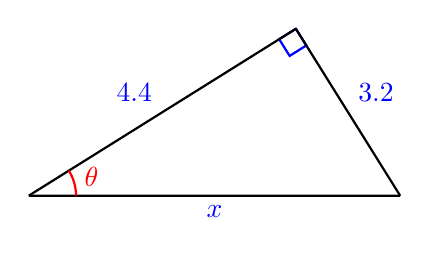
\begin{tikzpicture} [rotate=212]

\coordinate (O) at (0,0 );
\coordinate (A) at (4,0);
\coordinate (B) at (0,2.5);

\draw[blue,thick] (O) rectangle +(0.25,0.25);
\draw[black,thick](B)--(O) node[above right,midway] {\color{blue}$3.2$};
\draw[black,thick](A)--(B) node[below,midway] {\color{blue}$x$};
\draw[black,thick](A)--(O) node[above left,midway] {\color{blue}$4.4$};

\draw[red,thick] (A)++(-.6,0) arc(180:{180-atan(2.5/4)}:.6) node[right,midway, yshift=2]{\color{red}$\theta$};

\end{tikzpicture}
\newline

revchap2.21
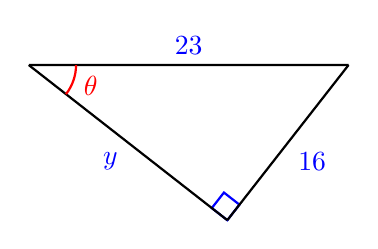
\begin{tikzpicture} [rotate=52]

\coordinate (O) at (0,0 );
\coordinate (A) at (2.5,0);
\coordinate (B) at (0,3.2);

\draw[blue,thick] (O) rectangle +(0.25,0.25);
\draw[black,thick](B)--(O) node[below left,midway] {\color{blue}$y$};
\draw[black,thick](A)--(B) node[above,midway] {\color{blue}$23$};
\draw[black,thick](A)--(O) node[below right,midway] {\color{blue}$16$};

\draw[red,thick] (B)++(0,-.6) arc(-90:{-atan(3.2/2.5)}:.6) node[right,midway, yshift=-2]{\color{red}$\theta$};

\end{tikzpicture}
\newline

revchap2.22
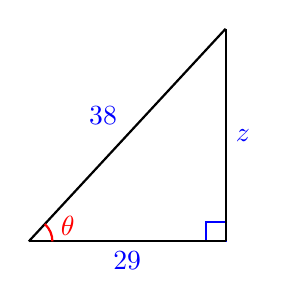
\begin{tikzpicture}

\coordinate (O) at (0,0 );
\coordinate (A) at (-2.5,0);
\coordinate (B) at (0,2.7);

\draw[blue,thick] (O) rectangle +(-0.25,0.25);
\draw[black,thick](B)--(O) node[right,midway] {\color{blue}$z$};
\draw[black,thick](A)--(B) node[above left,midway] {\color{blue}$38$};
\draw[black,thick](A)--(O)node[below,midway] {\color{blue}$29$};

\draw[red,thick] (A)++(.3,0) arc(0:{atan(2.7/2.5)}:.3) node[right,midway, yshift=2]{\color{red}$\theta$};

\end{tikzpicture}
\newline

revchap2.23
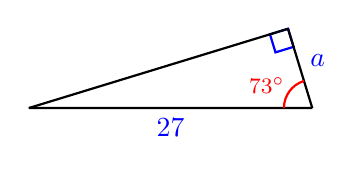
\begin{tikzpicture} [scale=1.2, rotate=197]

\coordinate (O) at (0,0 );
\coordinate (A) at (2.8689,0);
\coordinate (B) at (0,0.8771);

\draw[blue,thick] (O) rectangle +(0.2,0.2);
\draw[black,thick](B)--(O) node[above right,midway, yshift=-3] {\color{blue}$a$};
\draw[black,thick](A)--(B) node[below,midway] {\color{blue}$27$};
\draw[black,thick](A)--(O);

\draw[red,thick] (B)++(0,-.3) arc(-90:-17:.3) node[left,midway, xshift=2, yshift=2]{\footnotesize\color{red}$73\degree$};

\end{tikzpicture}
\newline

revchap2.24
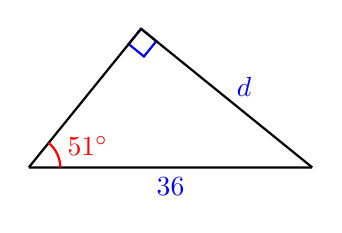
\begin{tikzpicture} [rotate=231]

\coordinate (O) at (0,0 );
\coordinate (A) at (2.26555,0);
\coordinate (B) at (0,2.7977);

\draw[blue,thick] (O) rectangle +(0.25,0.25);
\draw[black,thick](B)--(O) node[above right,midway, yshift=-3] {\color{blue}$d$};
\draw[black,thick](A)--(B) node[below,midway] {\color{blue}$36$};
\draw[black,thick](A)--(O);

\draw[red,thick] (A)++(-.4,0) arc(180:129:.4) node[right,midway,  yshift=3]{\color{red}$51\degree$};

\end{tikzpicture}
\newline

revchap2.25
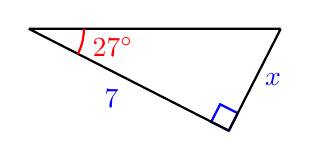
\begin{tikzpicture} [rotate=63]

\coordinate (O) at (0,0 );
\coordinate (A) at (1.453,0);
\coordinate (B) at (0,2.851);

\draw[blue,thick] (O) rectangle +(0.25,0.25);
\draw[black,thick](B)--(O) node[below left,midway] {\color{blue}$7$};
\draw[black,thick](A)--(B);
\draw[black,thick](A)--(O) node[right,midway] {\color{blue}$x$};

\draw[red,thick] (B)++(0,-.7) arc(-90:-63:.7) node[right,midway,  yshift=-2]{\color{red}$27\degree$};

\end{tikzpicture}
\newline

revchap2.26
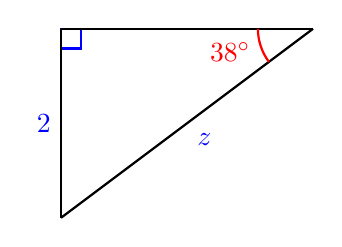
\begin{tikzpicture} 

\coordinate (O) at (0,0 );
\coordinate (A) at (3.2,0);
\coordinate (B) at (0,-2.4);

\draw[blue,thick] (O) rectangle +(0.25,-0.25);
\draw[black,thick](B)--(O) node[left,midway] {\color{blue}$2$};
\draw[black,thick](A)--(B) node[below right,midway] {\color{blue}$z$};
\draw[black,thick](A)--(O);

\draw[red,thick] (A)++(-.7,0) arc(180:{180+atan(2.4/3.2)}:.7) node[left,midway,  yshift=-2]{\color{red}$38\degree$};

\end{tikzpicture}
\newline

revchap2.27
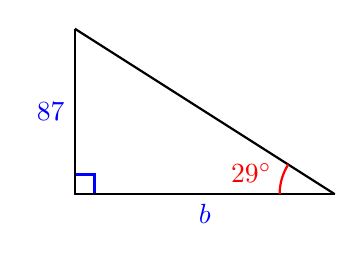
\begin{tikzpicture} 

\coordinate (O) at (0,0 );
\coordinate (A) at (3.3,0);
\coordinate (B) at (0,2.1);

\draw[blue,thick] (O) rectangle +(0.25,0.25);
\draw[black,thick](B)--(O) node[left,midway] {\color{blue}$87$};
\draw[black,thick](A)--(B);
\draw[black,thick](A)--(O) node[below,midway] {\color{blue}$b$};

\draw[red,thick] (A)++(-.7,0) arc(180:{180-atan(2.1/3.3)}:.7) node[left,midway,  yshift=2]{\color{red}$29\degree$};

\end{tikzpicture}
\newline

revchap2.28
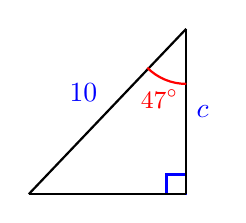
\begin{tikzpicture} 

\coordinate (O) at (0,0 );
\coordinate (A) at (-2,0);
\coordinate (B) at (0,2.1);

\draw[blue,thick] (O) rectangle +(-0.25,0.25);
\draw[black,thick](B)--(O) node[right,midway] {\color{blue}$c$};
\draw[black,thick](A)--(B) node[above left,midway] {\color{blue}$10$};
\draw[black,thick](A)--(O);

\draw[red,thick] (B)++(0,-.7) arc(270:{270-atan(2.1/2.1)}:.7) node[below,midway,  xshift=-2]{\small\color{red}$47\degree$};

\end{tikzpicture}
\newline

revchap2.29
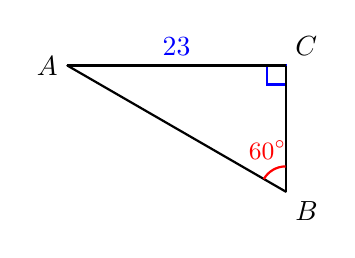
\begin{tikzpicture} [scale=1.6]

\coordinate (O) at (0,0 );
\coordinate (A) at (-1.732,0);
\coordinate (B) at (0,-1);

\filldraw[black] (O) circle (.1pt) node[anchor=south west] {$C$};
\filldraw[black] (A) circle (.1pt) node[anchor=east] {$A$};
\filldraw[black] (B) circle (.1pt) node[anchor=north west] {$B$};

\draw[blue,thick] (O) rectangle +(-0.15,-0.15);
\draw[black,thick](B)--(O);
\draw[black,thick](A)--(B);
\draw[black,thick](A)--(O) node[above,midway] {\color{blue}$23$};

\draw[red,thick] (B)++(0,.2) arc(90:150:.2) node[above,midway,  xshift=-2]{\small\color{red}$60\degree$};

\end{tikzpicture}
\newline

revchap2.30
\begin{tikzpicture}

\coordinate (C) at (0,0 );
\coordinate (A) at (-2.8,0);
\coordinate (B) at (0,-2.8);

\filldraw[black] (C) circle (.1pt) node[anchor=west] {$C$};
\filldraw[black] (A) circle (.1pt) node[anchor=east] {$A$};
\filldraw[black] (B) circle (.1pt) node[anchor=west] {$B$};

\draw[blue,thick] (O) rectangle +(-0.25,-0.25);
\draw[black,thick](B)--(O);
\draw[black,thick](A)--(B) node[below left,midway] {\color{blue}$14$};
\draw[black,thick](A)--(O);

\draw[red,thick] (B)++(0,.5) arc(90:135:.5) node[above,midway,  xshift=-2]{\small\color{red}$45\degree$};

\end{tikzpicture}
\newline

revchap2.31
\begin{tikzpicture}

\coordinate (C) at (0,0 );
\coordinate (D) at (-3.464,0);
\coordinate (E) at (2,0);
\coordinate (F) at (0,2);

\filldraw[black] (D) circle (.1pt) node[anchor=south, yshift=2] {$D$};
\filldraw[black] (E) circle (.1pt) node[anchor=south, yshift=2] {$E$};
\filldraw[black] (F) circle (.1pt) node[anchor=east, yshift=2] {$F$};

\draw[blue,thick] (O) rectangle +(-0.25,0.25);
\draw[black,thick] (D)--(E)--(F)--(D);
\draw[gray,thick, dashed] (C)--(F) node[left,midway] {\color{blue}$10$};

\draw[red,thick] (D)++(.5,0) arc(0:30:.5) node[right,midway,  yshift=2]{\small\color{red}$30\degree$};
\draw[red,thick] (E)++(-.4,0) arc(180:135:.4) node[left,midway,  yshift=2]{\small\color{red}$45\degree$};

\end{tikzpicture}
\newline

revchap2.32
\begin{tikzpicture}

\coordinate (C) at (0,0 );
\coordinate (D) at (0,2.4);
\coordinate (E) at (0,-1.386);
\coordinate (F) at (2.4,0);

\filldraw[black] (D) circle (.1pt) node[anchor=east] {$D$};
\filldraw[black] (E) circle (.1pt) node[anchor=east] {$E$};
\filldraw[black] (F) circle (.1pt) node[anchor=west] {$F$};

\draw[blue,thick] (O) rectangle +(0.25,0.25);
\draw[black,thick] (D)--(E)--(F)--(D);
\draw[gray,thick, dashed] (C)--(F) node[above,midway] {\color{blue}$12$};

\draw[red,thick] (D)++(0,-.5) arc(-90:-45:.5) node[below,midway,  xshift=4]{\small\color{red}$45\degree$};
\draw[red,thick] (E)++(0,.3) arc(90:30:.3) node[above,midway,  xshift=6]{\small\color{red}$60\degree$};

\end{tikzpicture}
\newline


revchap2.33
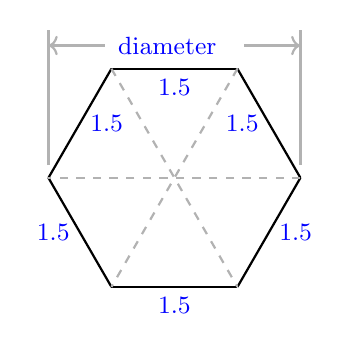
\begin{tikzpicture} [scale=.8]

\coordinate (O) at (0,0 );
\coordinate (A) at (2,0);
\coordinate (B) at (1,1.732);
\coordinate (C) at (-1,1.732);
\coordinate (D) at (-2,0);
\coordinate (E) at (-1,-1.732);
\coordinate (F) at (1,-1.732);

\draw[black,thick] (A)--(B) node[left,midway] {\small\color{blue}1.5};
\draw[black,thick] (C)--(B) node[below,midway] {\small\color{blue}1.5};
\draw[black,thick] (C)--(D) node[right,midway] {\small\color{blue}1.5};
\draw[black,thick] (D)--(E) node[left,midway] {\small\color{blue}1.5};
\draw[black,thick] (F)--(E) node[below,midway] {\small\color{blue}1.5};
\draw[black,thick] (F)--(A) node[right,midway] {\small\color{blue}1.5};

\draw[gray!60!white,thick, dashed] (A)--(D);
\draw[gray!60!white,thick, dashed] (B)--(E);
\draw[gray!60!white,thick, dashed] (C)--(F);

\draw[gray!60!white,thick] (D)++(0,.2)--+(0,2.15);
\draw[gray!60!white,thick] (A)++(0,.2)--+(0,2.15);
\draw[gray!60!white,thick, <-] (D)++(0,2.1)--+(.9,0) node[right, xshift=1] {\small\color{blue}diameter};
\draw[gray!60!white,thick, <-] (A)++(0,2.1)--+(-.9,0);

\end{tikzpicture}
\newline

revchap2.34
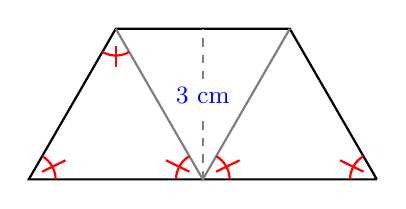
\begin{tikzpicture} [scale=.85]

\coordinate (O) at (0,0 );
\coordinate (A) at (2.6,0);
\coordinate (B) at (1.3,2.25);
\coordinate (C) at (-1.3,2.25);
\coordinate (D) at (-2.6,0);
\coordinate (E) at (0,2.25);

\draw[black,thick] (A)--(B)--(C)--(D)--(A);
\draw[gray,thick, dashed] (O)--(E) node[midway,fill=white, yshift=3] {\small\color{blue}3 cm};
\draw[gray,thick] (B)--(O)--(C);

\draw[red,thick] (D)++(.4,0) arc(0:60:.4);
\draw[red,thick] (D)++(.2,.115) -- +(.35,.17);

\draw[red,thick] (O)++(.4,0) arc(0:60:.4);
\draw[red,thick] (O)++(.2,.115) -- +(.35,.17);
\draw[red,thick] (O)++(-.4,0) arc(180:120:.4);
\draw[red,thick] (O)++(-.2,.115) -- +(-.35,.17);

\draw[red,thick] (A)++(-.4,0) arc(180:120:.4);
\draw[red,thick] (A)++(-.2,.115) -- +(-.35,.17);

\draw[red,thick] (C)++(-.2,-.346) arc(240:300:.4);
\draw[red,thick] (C)++(0,-.25) -- +(0,-.32);

\end{tikzpicture}
\newline



chap2rev35
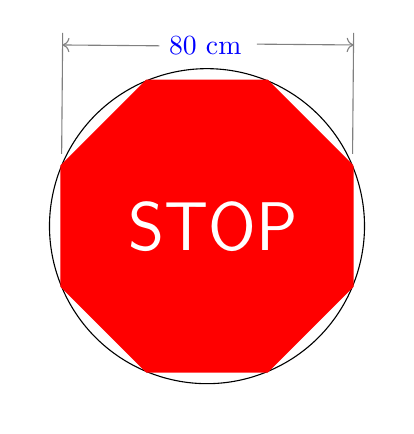
\begin{tikzpicture} [rotate=22.5]

\coordinate(O) at (0,0);
\coordinate (A) at (2,0 );
\coordinate (B) at (1.414,1.414);
\coordinate (C) at(0,2);
\coordinate (D) at (-1.414,1.414);
\coordinate (E) at(-2,0);
\coordinate (F) at(-1.414,-1.414);
\coordinate (G) at(0,-2);
\coordinate (H) at (1.414,-1.414);

\draw[black] (O) circle(2);

\draw[gray] (D)++(0.06,0.1414) -- +(.6,1.414);
\draw[gray, <-] (D)++(.6,1.414) -- +(1.131,-.48) node[right] {\color{blue}80 cm};
\draw[gray] (A)++(0.06,0.1414) -- +(.6,1.414);
\draw[gray, <-] (A)++(.6,1.414) -- +(-1.131,.48);

\filldraw[red,thick] (A)--(B)--(C)--(D)--(E)--(F)--(G)--(H)--(A);
\node [text width=2cm,font=\sffamily] at (O) {\Huge\color{white}STOP};

\end{tikzpicture}
\newline

chap2rev43
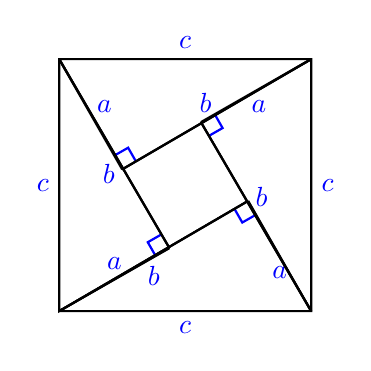
\begin{tikzpicture} 

\coordinate(O) at (0,0);
\coordinate (A) at (3.2,0 );
\coordinate (B) at (3.2,3.2);
\coordinate (C) at(0,3.2);
\coordinate (D) at (2.4,1.4);
\coordinate (E) at(1.8,2.4);
\coordinate (F) at(0.8,1.8);
\coordinate (G) at(1.4,0.8);

\draw[blue,thick] (D)++(-.175,-.1)--++(.1,-.175)--++(.175,.1);
\draw[blue,thick] (E)++(.1,-.175)--++(.175,.1)--++(-.1,.175);
\draw[blue,thick] (F)++(.175,.1)--++(-.1,.175)--++(-.175,-.1);
\draw[blue,thick] (G)++(-.1,.175)--++(-.175,-.1)--++(.1,-.175);

\draw[black, thick] (O)--(A) node[below,midway] {\color{blue}$c$};
\draw[black, thick] (B)--(A) node[right,midway] {\color{blue}$c$};
\draw[black, thick] (B)--(C) node[above,midway] {\color{blue}$c$};
\draw[black, thick] (O)--(C) node[left,midway] {\color{blue}$c$};

\draw[black, thick] (O)--(G) node[above,midway] {\color{blue}$a$};
\draw[black, thick] (O)--(D) node[below,midway] {\color{blue}$b$};

\draw[black, thick] (A)--(D) node[below,midway] {\color{blue}$a$};
\draw[black, thick] (A)--(E) node[above,midway, xshift=2] {\color{blue}$b$};

\draw[black, thick] (B)--(E) node[below,midway, xshift=1] {\color{blue}$a$};
\draw[black, thick] (B)--(F) node[above,midway,xshift=-4,yshift=-3] {\color{blue}$b$};

\draw[black, thick] (C)--(F) node[above,midway, xshift=5,yshift=-3] {\color{blue}$a$};
\draw[black, thick] (C)--(G) node[below,midway, xshift=-2] {\color{blue}$b$};

\draw[black, thick] (O)--(A)--(B)--(C)--(O)--(D);
\draw[black, thick] (A)--(E);
\draw[black, thick] (B)--(F);
\draw[black, thick] (C)--(G);


\end{tikzpicture}
\newline

chap2rev44
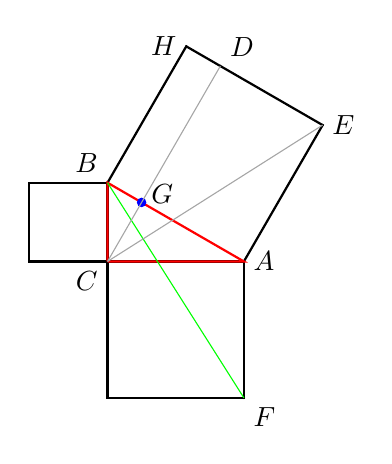
\begin{tikzpicture} 

\coordinate(C) at (0,0);
\coordinate (A) at (1.732,0 );
\coordinate (B) at (0,1);
\coordinate (D) at (1.433,2.482);
\coordinate (E) at(2.732,1.732);
\coordinate (F) at(1.732,-1.732);
\coordinate (G) at(0.433,0.75);
\coordinate (H) at(1,2.732);

\filldraw[black] (A) circle (0.2pt) node[anchor=west] {$A$};
\filldraw[black] (B) circle (0.2pt) node[anchor=south east] {$B$};
\filldraw[black] (C) circle (0.2pt) node[anchor=north east] {$C$};
\filldraw[black] (D) circle (0.2pt) node[anchor=south west] {$D$};
\filldraw[black] (E) circle (0.2pt) node[anchor=west] {$E$};
\filldraw[black] (F) circle (0.2pt) node[anchor=north west] {$F$};
\filldraw[black] (H) circle (0.2pt) node[anchor=east] {$H$};


\draw[black, thick] (A)--(E)--(H)--(B);
\draw[black, thick] (C) rectangle +(-1,1);
\draw[black, thick] (C) rectangle +(1.732,-1.732);
\draw[red, thick] (C)--(A)--(B)--(C);
\filldraw[blue] (G) circle (1.5pt) node[anchor=west, yshift=3] {\color{black}$G$};

\draw[green] (B)--(F);

\draw[gray!70!white] (C)--(E);
\draw[gray!70!white] (C)--(D);

\end{tikzpicture}
\newline










\section {Stuff for later}
Section 4.2 Angle of inclination
\begin{tikzpicture}

\coordinate (O) at (0,0);
\coordinate (x) at (3.5,0);
\coordinate (y) at (0,2);
\coordinate (A) at (3,1.8);
\coordinate (B) at (1.,0);
\coordinate (C) at (2.5,0);
\coordinate (D) at (-1,-1.8);

\draw[black,  thick, ->] (-1.5,0) --  (x) node[right] {$x$} ;
\draw[black,  thick, ->] (0,-2) --  (y) node[above] {$y$}  ;
\draw[black,  thick, <->] (D) --  (A)  ;
\draw[red, thick] (1.9,0) arc (0:{atan(0.9)}:.9) node [left, midway,xshift=0,yshift=-3] {$\alpha$};

\end{tikzpicture}
\newline

Section 4.2 Angle of inclination
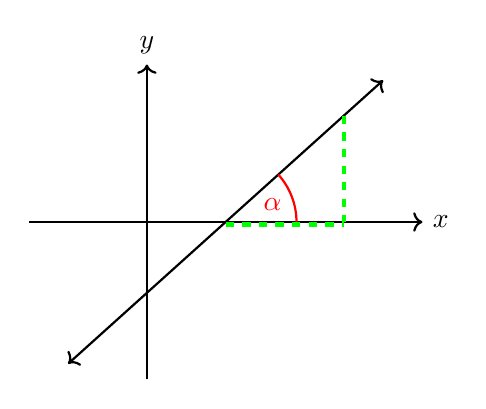
\begin{tikzpicture}

\coordinate (O) at (0,0);
\coordinate (x) at (3.5,0);
\coordinate (y) at (0,2);
\coordinate (A) at (3,1.8);
\coordinate (B) at (1.,0);
\coordinate (C) at (2.5,0);
\coordinate (D) at (-1,-1.8);

\draw[black,  thick, ->] (-1.5,0) --  (x) node[right] {$x$} ;
\draw[black,  thick, ->] (0,-2) --  (y) node[above] {$y$}  ;
\draw[black,  thick, <->] (D) --  (A)  ;
\draw[red, thick] (1.9,0) arc (0:{atan(0.9)}:.9) node [left, midway,xshift=0,yshift=-3] {$\alpha$};

\draw[green, ultra thick, dashed] (1,-.03) -- (2.5,-.03);
\draw[green, ultra thick, dashed] (2.5,1.35) -- (2.5,0);

\end{tikzpicture}
\newline


hp-2.1.21
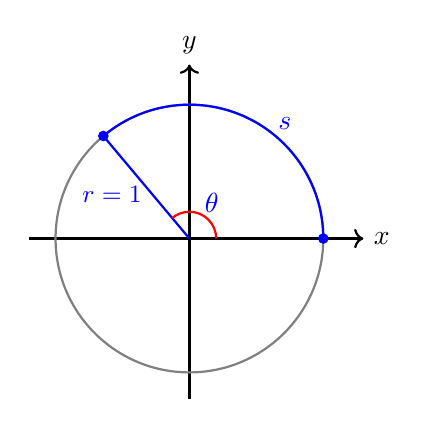
\begin{tikzpicture} [scale=1.7]

\draw[thick,->] (-1.2,0) -- (1.3,0) node[anchor=west] {$x$};
\draw[thick,->] (0,-1.2) -- (0,1.3) node[anchor=south] {$y$};

\coordinate(O) at (0,0);
\coordinate(A) at (1,0);
\coordinate (B) at (-.6428,0.766);

\draw[gray,thick] (O) circle (1);
\draw[blue,thick] (O) -- (B) node[below left, midway, xshift=2, yshift=4] {\small\color{blue} $r=1$};
\filldraw [blue] (A) circle (1pt);
\filldraw [blue] (B) circle (1pt);
\draw[blue,thick] (A) arc(0:130:1) node[above, midway, xshift=14, yshift=-8] {\color{blue}$s$};
\draw[red,thick] (O)++(.2,0) arc(0:130:.2) node[above, midway, xshift=4, yshift=-3] {\color{blue}$\theta$};

\end{tikzpicture}
\newline


Exercise not used?
\begin{tikzpicture}
\coordinate (O) at (0,0);
\coordinate (A) at (0,0);
\coordinate (B) at (0,0);
\coordinate(C) at (0,0);
\coordinate (D) at (0,0);
\filldraw[black] (O) circle (.2pt) node[anchor=south west, xshift=6]{$50\degree$};
\filldraw[black] (A) circle (.2pt) node[anchor=south east]{$x$};
\filldraw[black] (B) circle (.2pt) node[anchor=north east, xshift=-6]{$y$};
\filldraw[black] (C) circle (.2pt) node[anchor=north west]{$z$};
%\draw[black,  thick] (A) -- (B) --( C) -- cycle;
\draw[black] (-2.3,0) --  (2.3,0);
\draw[black] (0.8,1.3) --  (-0.8,-1.3) ;
\end{tikzpicture}
\newline


\end{document}
